\documentclass[12pt,a4paper]{article}

% -------------------- Packages --------------------
\usepackage[utf8]{inputenc}
\usepackage[T1]{fontenc}
\usepackage{lmodern}
\usepackage[a4paper,margin=25mm,headheight=15pt]{geometry}
\usepackage{amsmath,amssymb,mathtools}
\usepackage{graphicx}
\usepackage{xcolor}
\usepackage{booktabs}
\usepackage{tabularx}
\usepackage{array}
\usepackage{longtable}
\usepackage{float}
\usepackage{caption}
\usepackage{subcaption}
\usepackage{enumitem}
\usepackage{listings}
\usepackage{fancyhdr}
\usepackage{lastpage}
\usepackage{microtype}
\usepackage{setspace}
\usepackage{titlesec}
\usepackage[hidelinks]{hyperref}

% -------------------- Formatting --------------------
\definecolor{navy}{HTML}{17365D}
\definecolor{teal}{HTML}{087E8B}
\definecolor{lightblue}{HTML}{EAF2F8}
\definecolor{codegray}{HTML}{F4F6F7}
\definecolor{muted}{HTML}{555555}

\hypersetup{
  pdftitle={Polar Encoding and Decoding over an AWGN Channel},
  pdfauthor={Kshitiz Sinha, Himanshu Dubey, Pritika Mishra},
  pdfsubject={Polar-coded digital communication simulation}
}

\setstretch{1.14}
\setlength{\parskip}{5pt}
\setlength{\parindent}{0pt}
\setlist[itemize]{leftmargin=1.5em,itemsep=2pt,topsep=3pt}
\setlist[enumerate]{leftmargin=1.7em,itemsep=3pt,topsep=3pt}
\captionsetup{font=small,labelfont=bf}
\titleformat{\section}{\Large\bfseries\color{navy}}{\thesection}{0.7em}{}
\titleformat{\subsection}{\large\bfseries\color{teal}}{\thesubsection}{0.7em}{}
\titleformat{\subsubsection}{\normalsize\bfseries\color{navy}}{\thesubsubsection}{0.7em}{}
\titlespacing*{\section}{0pt}{17pt}{7pt}
\titlespacing*{\subsection}{0pt}{12pt}{5pt}

\pagestyle{fancy}
\fancyhf{}
\lhead{\small Polar Coding over AWGN}
\rhead{\small Assignment Report}
\cfoot{\small Page \thepage\ of \pageref{LastPage}}
\renewcommand{\headrulewidth}{0.4pt}

\newcolumntype{Y}{>{\raggedright\arraybackslash}X}
\newcommand{\code}[1]{\texttt{#1}}
\newcommand{\placeholder}[2]{%
  \fbox{\begin{minipage}[c][0.32\textheight][c]{0.91\linewidth}
    \centering\color{muted}\textbf{#1}\\[6pt]
    #2\\[6pt]
    \small Add your original screenshot as \code{#1} in the \code{figures/} folder.
  \end{minipage}}}
\newcommand{\appendixshot}[3]{%
  \begin{figure}[H]
    \centering
    \IfFileExists{figures/#1}{\includegraphics[width=0.92\linewidth,height=0.33\textheight,keepaspectratio]{figures/#1}}{\placeholder{#1}{#3}}
    \caption{#2}
  \end{figure}}

\begin{document}

% ==================== Cover page ====================
\hypersetup{pageanchor=false}
\begin{titlepage}
  \centering
  \vspace*{0.45cm}

  {\Large\bfseries GROUP ASSIGNMENT REPORT\par}
  \vspace{0.30cm}
  {\large\bfseries INFORMATION THEORY AND CODING (ITC)\par}
  \vspace{0.12cm}
  {\normalsize Subject Code: EC24309\par}

  \vspace{0.70cm}
  {\Huge\bfseries\color{navy} Polar Encoding and Decoding\par}
  \vspace{0.20cm}
  {\LARGE\bfseries over an AWGN Channel\par}
  \vspace{0.25cm}
  {\large End-to-end text transmission using BPSK and Successive Cancellation decoding\par}

  \vspace{0.45cm}
  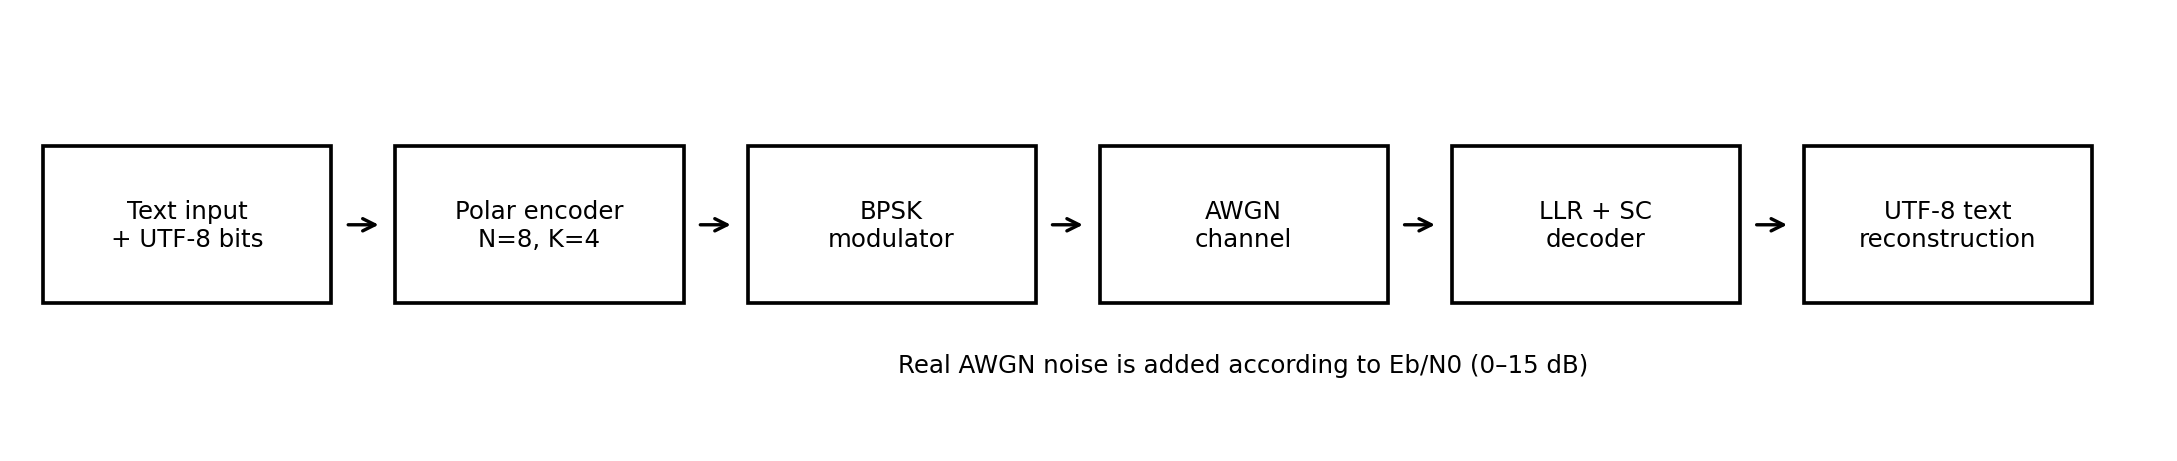
\includegraphics[width=0.92\linewidth,height=0.23\textheight,keepaspectratio]{figures/system_diagram.png}
  \vspace{0.30cm}

  {\large\bfseries GROUP MEMBERS\par}
  \vspace{0.16cm}
  \renewcommand{\arraystretch}{1.35}
  \begin{tabularx}{0.90\linewidth}{c >{\raggedright\arraybackslash}X >{\centering\arraybackslash}p{0.31\linewidth}}
    \toprule
    \textbf{S. No.} & \textbf{Name} & \textbf{Roll Number}\\
    \midrule
    1 & Kshitiz Sinha & BTECH/10686/24\\
    2 & Himanshu Dubey & BTECH/10682/24\\
    3 & Pritika Mishra & BTECH/10671/24\\
    \bottomrule
  \end{tabularx}

  \vspace{0.35cm}
  \renewcommand{\arraystretch}{1.28}
  \begin{tabularx}{0.90\linewidth}{>{\bfseries}p{0.29\linewidth}Y}
    Branch & Electronics and Communication Engineering (ECE)\\
    Section & C\\
    Subject & Information Theory and Coding (ITC)\\
    Subject Code & EC24309\\
    Submitted to & Dr. Sanjeet Kumar\\
    Institution & Birla Institute of Technology, Mesra\\
    Submission Date & 4th October 2026\\
  \end{tabularx}

  \vfill
\end{titlepage}

\hypersetup{pageanchor=true}
\pagenumbering{roman}
\tableofcontents
\clearpage
\listoffigures
\clearpage
\pagenumbering{arabic}

% ==================== Abstract ====================
\section*{Abstract}
\addcontentsline{toc}{section}{Abstract}
This assignment implements and studies a short Polar-coded digital communication link over an additive white Gaussian noise (AWGN) channel. A user-entered UTF-8 message is converted into bits, framed with a 16-bit payload-length header, divided into 4-bit information blocks, and encoded using an $(N=8,K=4)$ Polar code. Each codeword is mapped to BPSK symbols and transmitted through an AWGN channel at $E_b/N_0$ values from 0 dB to 15 dB. At the receiver, channel log-likelihood ratios (LLRs) are calculated and a recursive Successive Cancellation (SC) decoder estimates the information bits. The decoded stream is reconstructed as UTF-8 text. A Monte Carlo experiment using 1,200 frames per SNR point measures bit error rate (BER) and frame error rate (FER). The measured errors decrease as $E_b/N_0$ increases; no errors were observed in the finite simulation runs from 7 dB to 15 dB.

\subsection*{Objectives}
\phantomsection\addcontentsline{toc}{subsection}{Objectives}
\begin{itemize}
  \item Implement Polar encoding with frozen-bit insertion and the Ar\i kan transform over $GF(2)$.
  \item Transmit encoded bits using BPSK modulation through a simulated AWGN channel.
  \item Implement soft-input recursive Successive Cancellation decoding using the $f$ and $g$ LLR updates.
  \item Demonstrate variable-length UTF-8 message transmission and reconstruction.
  \item Evaluate BER and FER over $E_b/N_0$ values from 0 dB to 15 dB.
\end{itemize}

% ==================== Introduction ====================
\section{Introduction}
Channel coding adds structured redundancy to transmitted data so that a receiver can detect and correct some errors caused by a noisy communication channel. Polar codes are a class of linear block codes based on channel polarization. They transform a group of input bits into a codeword while assigning selected input positions to information bits and fixing the remaining positions to known frozen values. The receiver uses the received channel observations to estimate the original information bits.

This project demonstrates the complete process in software. It is an educational, small-block implementation designed to make intermediate vectors, channel samples, and decoder decisions visible. The selected construction is not intended to represent the rate-matching and reliability-sequence procedures of a standards-compliant 5G New Radio (NR) Polar code.

% ==================== Theory ====================
\section{Theoretical Background}
\subsection{Polar transform and frozen bits}
The basic Polar kernel is the binary matrix
\begin{equation}
  F = \begin{bmatrix} 1 & 0 \\ 1 & 1 \end{bmatrix}.
  \label{eq:kernel}
\end{equation}
For a block length $N=2^m$, the generator matrix is the $m$-fold Kronecker product of $F$:
\begin{equation}
  G_N = F^{\otimes m}, \qquad N=2^m.
  \label{eq:generator}
\end{equation}
Encoding is performed over $GF(2)$, where addition is equivalent to XOR:
\begin{equation}
  \mathbf{x}=\mathbf{u}G_N\pmod 2.
  \label{eq:encoding}
\end{equation}

The input vector $\mathbf{u}$ contains $N$ positions. In this assignment, $N=8$ and $K=4$. The four information bits are placed at zero-based positions $[3,5,6,7]$; the frozen positions $[0,1,2,4]$ are set to zero. The encoder applies the Polar transform to produce an 8-bit codeword.

\begin{table}[H]
\centering
\caption{Polar code configuration used in the simulation.}
\label{tab:codeparams}
\begin{tabularx}{0.82\linewidth}{lY}
\toprule
\textbf{Parameter} & \textbf{Value}\\
\midrule
Block length ($N$) & 8\\
Information bits ($K$) & 4\\
Frozen bits ($N-K$) & 4\\
Code rate ($R=K/N$) & 0.5\\
Information positions (zero-based) & $[3,5,6,7]$\\
Frozen positions (zero-based) & $[0,1,2,4]$\\
\bottomrule
\end{tabularx}
\end{table}

\subsection{BPSK modulation}
Each encoded bit is mapped to a real-valued BPSK symbol with unit energy:
\begin{equation}
  0\mapsto +1, \qquad 1\mapsto -1.
  \label{eq:bpsk}
\end{equation}

\subsection{AWGN channel and noise variance}
The channel adds a zero-mean Gaussian random sample to each transmitted symbol. The received sample is
\begin{equation}
  y=s+n, \qquad n\sim\mathcal{N}(0,\sigma^2),
  \label{eq:awgn}
\end{equation}
where $s$ is the transmitted symbol, $n$ is independent Gaussian noise, and $\sigma^2$ is the noise variance. $E_b/N_0$ is expressed per information bit. With unit-energy BPSK and code rate $R$, the real-valued noise variance used by the program is
\begin{equation}
  \sigma^2=\frac{1}{2R\,10^{(E_b/N_0)_{\mathrm{dB}}/10}},
  \qquad R=\frac{K}{N}.
  \label{eq:noisevariance}
\end{equation}
For this code, $R=1/2$. Increasing $E_b/N_0$ reduces the noise variance, so the received samples tend to be closer to the transmitted BPSK symbols.

\subsection{Channel log-likelihood ratio}
The receiver converts each noisy BPSK observation into a log-likelihood ratio. Under the mapping $0\mapsto +1$ and $1\mapsto -1$, a positive LLR favours coded bit 0:
\begin{equation}
  L(y)=\log\frac{p(y\mid x=0)}{p(y\mid x=1)}
      =\frac{2y}{\sigma^2}.
  \label{eq:llr}
\end{equation}

\subsection{Successive Cancellation decoding}
The recursive SC decoder uses soft information to estimate the input bits in their decoding order. The $f$ operation combines LLRs to decode the first half of a constituent block. The $g$ operation uses previously decoded partial sums to calculate LLRs for the second half. At frozen positions, the decoder forces the decision to zero; at information positions, the sign of the LLR determines the hard decision.
\begin{align}
  f(a,b) &= 2\tanh^{-1}\!\left(\tanh\frac{a}{2}\;\tanh\frac{b}{2}\right),
  \label{eq:fupdate}\\
  g(a,b,\hat{u}) &= b+(1-2\hat{u})a.
  \label{eq:gupdate}
\end{align}
The implementation evaluates the $f$ update using a numerically stable log-domain expression and evaluates the $g$ update using the decoded partial sums from the left branch.

% ==================== Workflow ====================
\section{Program Workflow}
The sequence shown in Figure~\ref{fig:system} is repeated block-by-block: the framed bitstream is divided into 4-bit information blocks, and each block is independently encoded into an 8-bit codeword before modulation and transmission.

\begin{figure}[H]
  \centering
  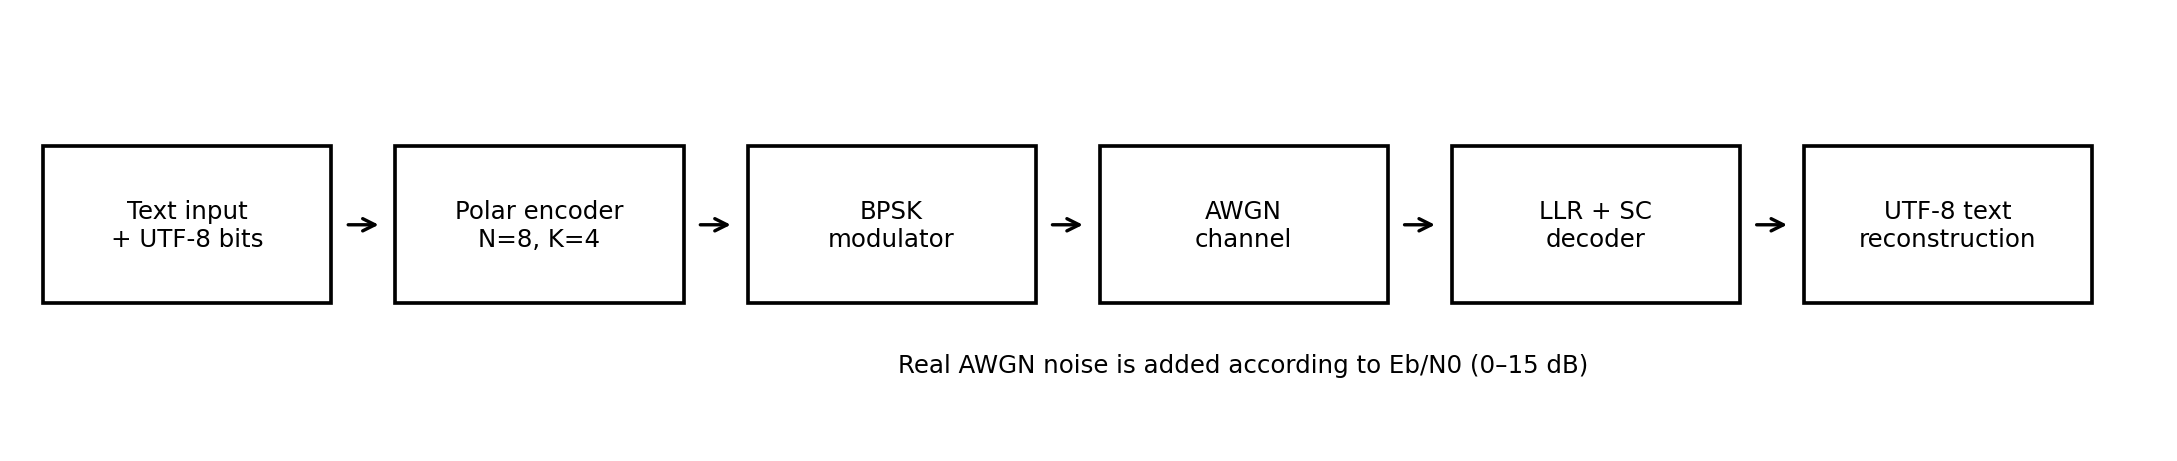
\includegraphics[width=\linewidth]{figures/system_diagram.png}
  \caption{Functional block diagram of the simulated transmitter--channel--receiver chain.}
  \label{fig:system}
\end{figure}

\begin{enumerate}
  \item \textbf{Message entry and UTF-8 conversion:} The user enters text. The program encodes it as UTF-8 bytes and converts each byte into eight bits.
  \item \textbf{Framing:} A 16-bit header containing the payload length in bytes is prepended. Zero padding is appended, if required, so the bitstream length is divisible by $K=4$.
  \item \textbf{Block formation:} The framed stream is divided into 4-bit information blocks.
  \item \textbf{Polar encoding:} For each block, four information bits are inserted at positions $[3,5,6,7]$ in an 8-bit vector; the frozen positions are zero. The Polar transform creates an 8-bit codeword.
  \item \textbf{BPSK and AWGN:} Code bits are mapped to $+1/-1$ symbols. Independent Gaussian noise is added using the selected $E_b/N_0$ value.
  \item \textbf{Soft demodulation and decoding:} The receiver computes channel LLRs and applies the recursive SC decoder to each codeword.
  \item \textbf{Message reconstruction:} Decoded information blocks are concatenated. The receiver reads the length header, removes padding, rebuilds the payload bytes, and decodes them as UTF-8 text.
\end{enumerate}

\subsection{Variable-length message support}
The 4-bit information size is the size of each Polar input block, not the maximum length of the user message. A longer text is converted into a longer bitstream and split across as many 4-bit blocks as necessary. The 16-bit length header supports payloads up to 65,535 UTF-8 bytes. The message is reconstructed only if the relevant decoded bits, including the header, are recovered correctly.

% ==================== Implementation ====================
\section{Software Implementation}
The project is implemented in Python. NumPy handles binary arrays, numerical operations, and random Gaussian samples. Matplotlib generates the performance plots. Streamlit provides the interactive user interface. Pytest is used for automated checks.

\begin{table}[H]
\centering
\caption{Main project files and their responsibilities.}
\label{tab:files}
\small
\begin{tabularx}{\linewidth}{>{\raggedright\arraybackslash}p{0.27\linewidth}Y}
\toprule
\textbf{File} & \textbf{Purpose}\\
\midrule
\code{app.py} & Streamlit interface for message transmission, detailed block inspection, BER/FER simulation, and theory.\\
\code{polar\_code.py} & Polar transform, information/frozen-bit placement, recursive SC decoding, and channel LLR calculation.\\
\code{channel.py} & BPSK modulation, $E_b/N_0$-to-noise-variance conversion, and AWGN generation.\\
\code{text\_codec.py} & UTF-8 conversion, 16-bit payload-length header, padding, and message reconstruction.\\
\code{transmission.py} & Coordinates end-to-end message framing, encoding, transmission, decoding, and reconstruction.\\
\code{performance.py} & Monte Carlo simulation of BER and FER over the selected SNR values.\\
\code{test\_core.py} & Automated checks for noiseless recovery of all 16 messages and encoder dimensions/bit placement.\\
\code{sionna\_verify.py} & Optional reference-check script; it is not required to run the custom application.\\
\bottomrule
\end{tabularx}
\end{table}

% ==================== Experimental setup ====================
\section{Experimental Setup}
\begin{table}[H]
\centering
\caption{Simulation parameters.}
\label{tab:simparams}
\begin{tabularx}{0.9\linewidth}{lY}
\toprule
\textbf{Setting} & \textbf{Value}\\
\midrule
Polar block length ($N$) & 8\\
Information bits per block ($K$) & 4\\
Code rate & $1/2$\\
Modulation & BPSK\\
Channel & Real AWGN\\
Decoder & Recursive Successive Cancellation\\
$E_b/N_0$ sweep & 0 dB to 15 dB, in 1 dB steps\\
Frames per SNR point & 1,200\\
Information bits per SNR point & 4,800\\
Performance experiment seed & Application default: 2026 (unless changed)\\
\bottomrule
\end{tabularx}
\end{table}

For each SNR point, 1,200 random 4-bit information frames were encoded and transmitted. Thus, 4,800 information bits were evaluated at every SNR point. A frame is counted as erroneous if at least one of its four decoded information bits differs from the transmitted information bits.

The error rates are calculated as
\begin{equation}
  \mathrm{BER}=\frac{\text{number of erroneous information bits}}{4800},
  \qquad
  \mathrm{FER}=\frac{\text{number of erroneous frames}}{1200}.
  \label{eq:errorrates}
\end{equation}

% ==================== Results ====================
\section{Simulation Results}
The following table records the measured results from the Streamlit BER/FER experiment. BER is the number of erroneous information bits divided by 4,800. FER is the number of erroneous frames divided by 1,200.

\begin{table}[H]
\centering
\caption{Measured BER and FER for the Polar-coded BPSK system.}
\label{tab:results}
\small
\setlength{\tabcolsep}{6pt}
\begin{tabular}{r r r r r}
\toprule
\textbf{$E_b/N_0$ (dB)} & \textbf{Bit errors} & \textbf{Frame errors} & \textbf{BER} & \textbf{FER}\\
\midrule
0  & 427 & 202 & 0.0889583  & 0.168333\\
1  & 305 & 135 & 0.0635417  & 0.112500\\
2  & 165 & 73  & 0.0343750  & 0.0608333\\
3  & 60  & 27  & 0.0125000  & 0.022500\\
4  & 28  & 14  & 0.00583333 & 0.0116667\\
5  & 6   & 3   & 0.00125000 & 0.002500\\
6  & 5   & 2   & 0.00104167 & 0.00166667\\
7  & 0   & 0   & 0          & 0\\
8  & 0   & 0   & 0          & 0\\
9  & 0   & 0   & 0          & 0\\
10 & 0   & 0   & 0          & 0\\
11 & 0   & 0   & 0          & 0\\
12 & 0   & 0   & 0          & 0\\
13 & 0   & 0   & 0          & 0\\
14 & 0   & 0   & 0          & 0\\
15 & 0   & 0   & 0          & 0\\
\bottomrule
\end{tabular}
\end{table}

\subsection{BER versus \texorpdfstring{$E_b/N_0$}{Eb/N0}}
\begin{figure}[H]
  \centering
  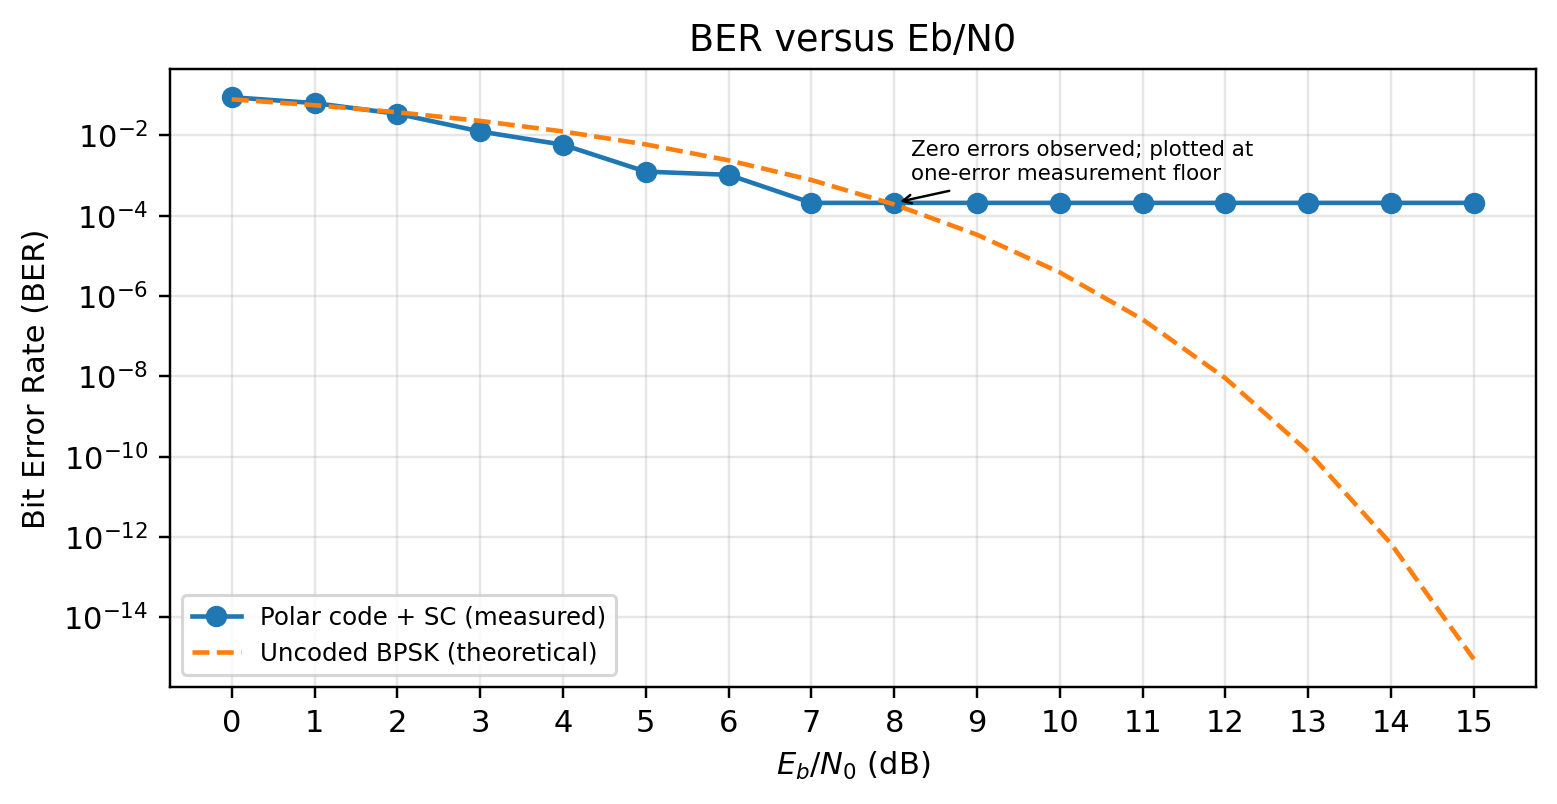
\includegraphics[width=0.94\linewidth]{figures/ber_plot.png}
  \caption{Measured Polar-coded BER and theoretical uncoded BPSK reference versus \texorpdfstring{$E_b/N_0$}{Eb/N0}.}
  \label{fig:ber}
\end{figure}
The measured BER decreases from 0.0889583 at 0 dB to 0.00104167 at 6 dB. No information-bit errors were observed in the 1,200-frame runs at SNR values from 7 dB through 15 dB. The plot uses a one-error measurement floor ($1/4800$) for zero-count points because a logarithmic axis cannot display zero. The table retains the measured value of zero.

\subsection{FER versus \texorpdfstring{$E_b/N_0$}{Eb/N0}}
\begin{figure}[H]
  \centering
  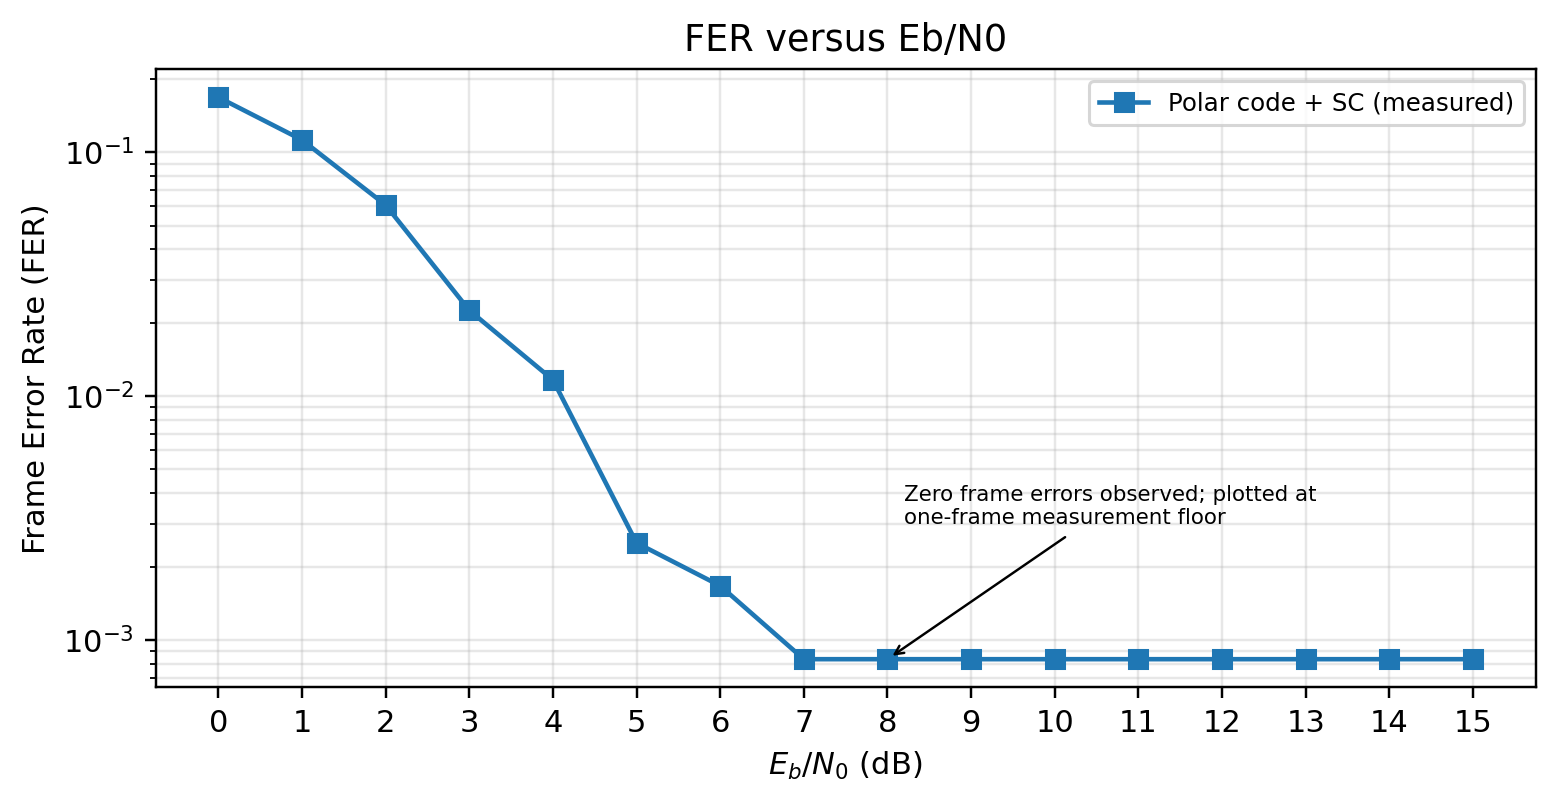
\includegraphics[width=0.94\linewidth]{figures/fer_plot.png}
  \caption{Measured Polar-coded FER versus \texorpdfstring{$E_b/N_0$}{Eb/N0}.}
  \label{fig:fer}
\end{figure}
The measured FER decreases from 0.168333 at 0 dB to 0.00166667 at 6 dB. No erroneous frames were observed from 7 dB through 15 dB in the finite runs. The logarithmic plot places zero-count points at the one-frame measurement floor ($1/1200$); this is a plotting convention, not a measured nonzero error rate.

\subsection{End-to-end message transmission tests}
Four of the five demonstration messages were recovered exactly. The 0 dB test failed to reconstruct the original message. At low $E_b/N_0$, noise can cause information-bit errors or corrupt the decoded length header, preventing valid UTF-8 reconstruction. This demonstrates that message recovery depends on the quality of the noisy channel.

\begin{table}[H]
\centering
\caption{Observed outcomes of the message transmission demonstration.}
\label{tab:message-tests}
\begin{tabularx}{\linewidth}{l l Y}
\toprule
\textbf{Test message} & \textbf{$E_b/N_0$} & \textbf{Observed outcome}\\
\midrule
HI & 15 dB & Recovered successfully\\
HELLO WORLD & 10 dB & Recovered successfully\\
English sentence & 8 dB & Recovered successfully\\
Hindi UTF-8 message & 15 dB & Recovered successfully\\
HELLO WORLD & 0 dB & Exact recovery failed\\
\bottomrule
\end{tabularx}
\end{table}

% ==================== Discussion ====================
\section{Discussion}
The overall BER and FER trends decrease as $E_b/N_0$ increases, which is consistent with the reduction in AWGN variance at higher $E_b/N_0$.
\begin{itemize}
  \item At 0 dB, 427 information-bit errors and 202 erroneous frames were observed out of 4,800 bits and 1,200 frames, respectively.
  \item At 5 dB, the measured BER was 0.00125 and FER was 0.0025. At 6 dB, the measured BER was 0.00104167 and FER was 0.00166667.
  \item From 7 dB to 15 dB, the finite experiment observed zero bit errors and zero frame errors. This does not establish that the true BER or FER is exactly zero; more frames are needed to estimate rarer errors.
  \item The message demonstration complements the Monte Carlo experiment: it shows a user-entered payload passing through framing, block encoding, modulation, noise, decoding, and text reconstruction.
\end{itemize}

% ==================== Validation ====================
\section{Software Validation}
The project test suite was run using the command:
\begin{lstlisting}[basicstyle=\ttfamily\small,backgroundcolor=\color{codegray},frame=single,breaklines=true]
python -m pytest test_core.py -v
\end{lstlisting}
The observed test output was \textbf{2 passed in 0.32 seconds}. The project directory structure was also inspected and verified by the user.

\begin{table}[H]
\centering
\caption{Automated test summary.}
\label{tab:tests}
\small
\begin{tabularx}{\linewidth}{>{\raggedright\arraybackslash}p{0.34\linewidth}YY}
\toprule
\textbf{Automated test} & \textbf{Purpose} & \textbf{Observed result}\\
\midrule
\shortstack[l]{\code{test\_all\_16\_messages\_}\\\code{decode\_without\_noise}} & Checks that all $2^K=16$ possible 4-bit information messages are recovered by the SC decoder when supplied with high-confidence, noiseless channel LLRs. & PASS\\
\shortstack[l]{\code{test\_encoder\_returns\_}\\\code{correct\_lengths}} & Checks that the encoder returns an $N=8$ input vector and $N=8$ codeword, and that information bits occupy the configured positions. & PASS\\
\bottomrule
\end{tabularx}
\end{table}
These tests verify core encoder/decoder properties; they are not an exhaustive proof of performance under every noise condition.

% ==================== Limitations ====================
\section{Limitations and Future Improvements}
\begin{itemize}
  \item The code uses a short $N=8$, $K=4$ educational construction with a fixed information set. It is not a 5G NR-compliant Polar code construction.
  \item The BER/FER experiment uses a finite sample of 1,200 frames per SNR point. More frames, especially at higher SNR, are needed to resolve very low error probabilities.
  \item The system does not include a CRC, retransmission protocol, channel interleaving, or practical synchronization and channel estimation.
  \item The current implementation uses one fixed block configuration. Larger Polar block lengths and a reliability-based information set could be implemented as an extension.
  \item An optional Sionna reference script is included, but the results in this report come from the custom NumPy implementation and do not claim an independent Sionna cross-check.
\end{itemize}

% ==================== Conclusion ====================
\section{Conclusion}
An end-to-end Polar-coded communication simulation over an AWGN channel was implemented in Python. The system accepts variable-length UTF-8 text, frames it with a payload-length header, encodes the bitstream in 4-bit information blocks using an $(8,4)$ Polar code, performs BPSK modulation, adds Gaussian noise, and recovers the text using a recursive SC decoder. The Monte Carlo results show decreasing BER and FER as $E_b/N_0$ increases from 0 dB to 15 dB. In the 1,200-frame experiments, no errors were observed from 7 dB onwards, while the message tests showed that low-SNR noise can prevent exact reconstruction. The assignment therefore demonstrates both the encoding/decoding workflow and the effect of channel SNR on communication reliability.

% ==================== References ====================
\section*{References}
\addcontentsline{toc}{section}{References}
\begin{enumerate}[label={[\arabic*]}]
  \item E. Ar\i kan, ``Channel polarization: A method for constructing capacity-achieving codes for symmetric binary-input memoryless channels,'' \emph{IEEE Transactions on Information Theory}, vol. 55, no. 7, pp. 3051--3073, July 2009, doi: 10.1109/TIT.2009.2021379.
  \item Project implementation and experimental output: custom Python/NumPy Polar encoder, recursive SC decoder, BPSK/AWGN simulation, and Streamlit interface developed for this assignment.
\end{enumerate}

% ==================== Appendix ====================
\clearpage
\appendix
\section{Application Screenshots}
Insert screenshots captured directly from the running Streamlit application. The LaTeX source automatically includes a screenshot when a file with the indicated name is placed in the \code{figures/} folder. Otherwise, a labelled placeholder is shown.

\appendixshot{screenshot-message.png}{Message transmission: original message, selected $E_b/N_0$, and recovered output.}{Show the message entered at the sender and the receiver's recovered text.}
\appendixshot{screenshot-blocks.png}{Block inspection: information bits, frozen-bit vector, codeword, BPSK symbols, AWGN samples, received values, LLRs, and SC decisions.}{Show at least one expanded transmission block.}
\clearpage
\appendixshot{screenshot-ber-app.png}{BER versus $E_b/N_0$ graph from the running application.}{Show the BER plot generated by Streamlit.}
\appendixshot{screenshot-fer-table.png}{FER versus $E_b/N_0$ graph and the numerical results table.}{Show the FER plot and measured result table.}

\end{document}
